We have make several attempts to adapt existing mechanism into our model.
\subsection{DNA on connected network}
One of the outstanding work on double auction on social network is Double Network Auction (DNA)
[need cite](DNA-Junping Xu). The methods is an extension of McAfee's trade reduction mechanism
runs on several disjoint buyer networks. Therefore, we may try to reduce our problem to use DNA
by dividing our connect buyer networks into several disjoint buyer network according to the allocation, we can then use DNA. However, we can find there exists situation when the network is individable. Figure \ref*{fig:DNACounter}
shows one of the situation when several sellers together connected to a chain of buyers. Therefore,
our problem setting cannot be reduced.
\begin{figure}[htbp]
  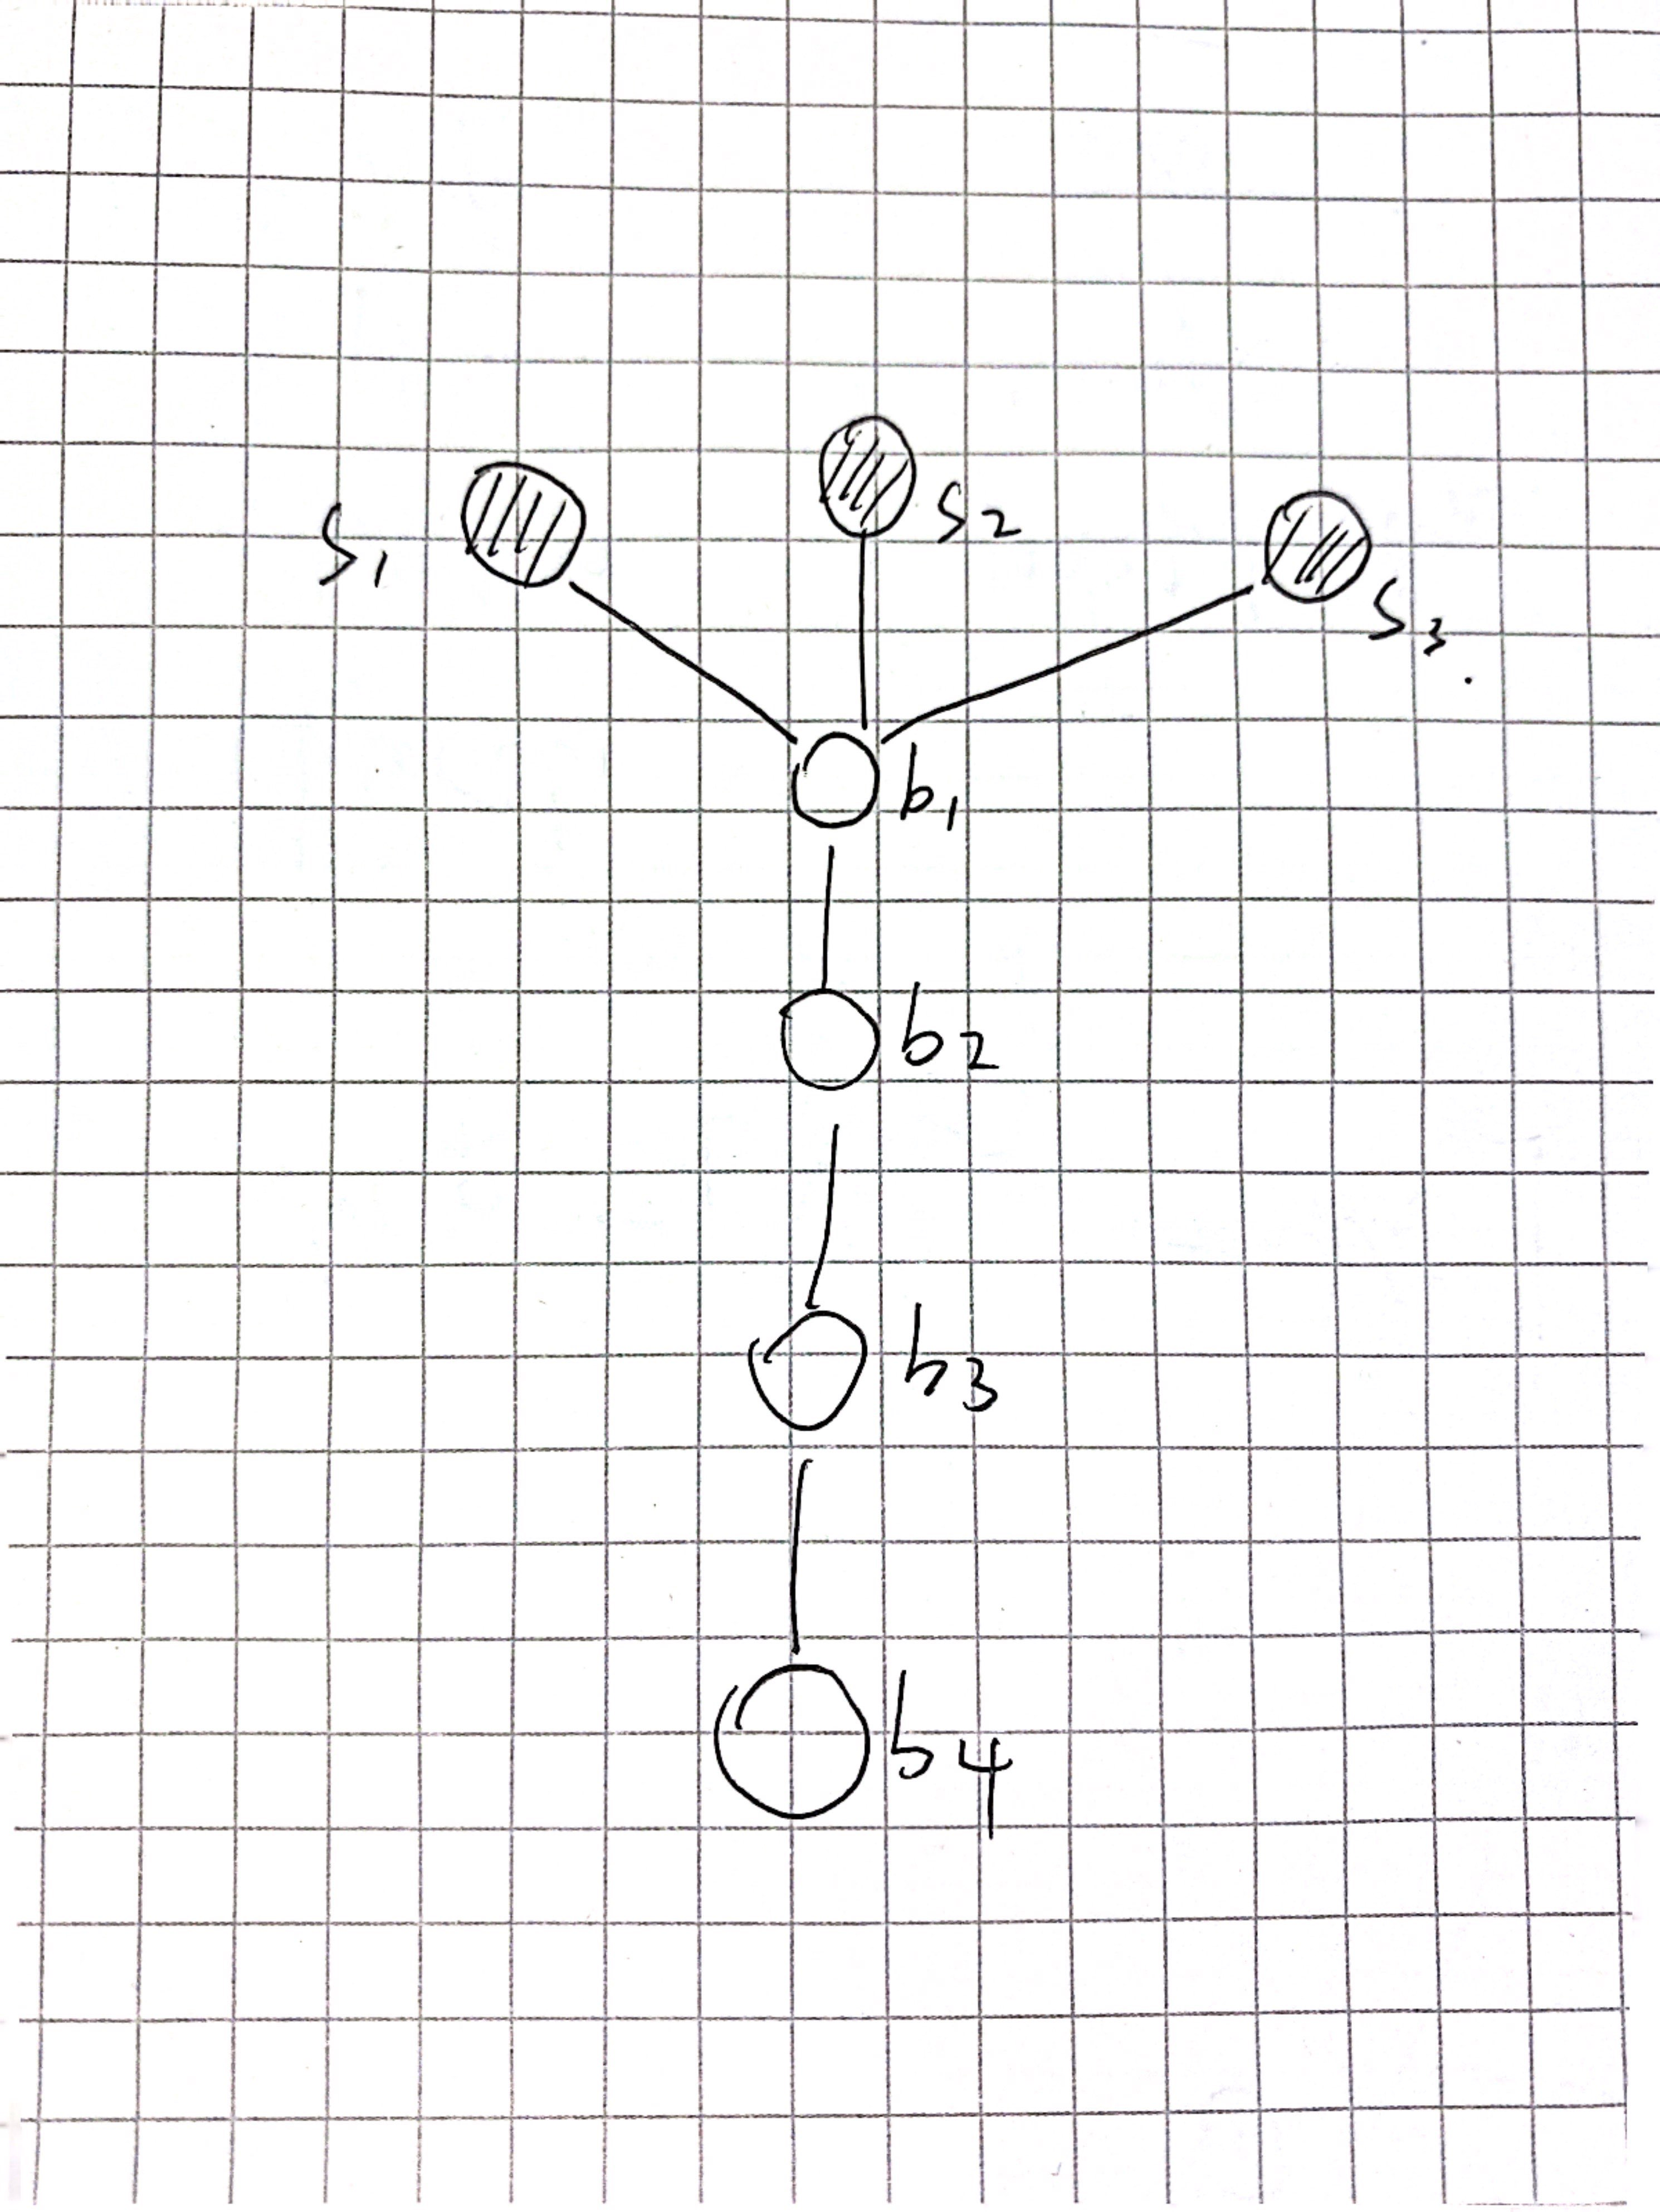
\includegraphics[scale = 0.05]{./figure/DNA_counter_1.jpg}
  \caption{Network that can not be divided}
  \label{fig:DNACounter}
\end{figure}
\subsection{multi-item mechanism}
In double auction scenario, we have multiple sellers, which means we also have multiple items. Therefore,
multi-item mechanism may provide some useful insights.\par
First, we try to adapt Generalized IDM(GIDM) and Distance-based Network Auction mechanism for Multi-unit, Unit-demand buyers(DNA-MU).
However, this two methods are not IC. The counter example are given in \ref*{need figure}. We can reduce our problem to a multi-item problem if we connect several sellers to the same buyer with identical price. It can be expected that our
adapted method will not be IC either.\par
We also look into two other IC mechanisms: MUDAN and LDM. These two methods are both layer-based mechanism.
In our setting, items are hold by different sellers. If the sellers are scattered around the network, then the
network will degenerate into one layer network, since the children have no chance to get the even they may have higher
evaluation.
\subsection*{Resale mechanism with leave and share}
In double-auction, we want people with high valuation hold the item. Therefore, resale mechanisms are better than
layer-based mechanism. Buyers with highre evaluation have more chance to get the item, while buyers with lower
evaluation are rewarded if they invite someone who get the item. From this insight, we designed a naive
resale mechanism combined IDM with leave and share. The mechanism is described as follows,
\begin{enumerate}
  \item Sort the sellers in order of their price from lowest to highest.
  \item Let the seller with lowest price sell the item, using IDM. Other sellers are viewed as buyer with 0 valuation.
  \item The seller and the winner leave the network and share their connection.
  \item Repeat step 2, 3 until no seller can sell the item.
\end{enumerate}
However, this mechanism is not IC, since seller with lower price have more chance to sell their
item with a high price, seller has the incentive to misreport a lower price. In the following example,
[exaple]
\subsection*{Resale with leave and share, eliminating highest \(m\) bid}
Then we made a modification to the original algorithm. The main idea is still the same, but when calculating
the price using IDM, we first eliminating the highest \(m\) bids, where \(m\) is the number of the unmatched seller.
As a result, the seller cannot get more profit by misreport, so does the buyer. However we still have to do
more work to show and prove this mechanism is IC.
Moreover, Since we have eliminated the highest bids, some deals that might have worked will fail. [example]
This will not be the problem if the network is big and the number of the buyer is much greater than the seller.